\subsection{Monolithic architecture}
In the beggining of the internet, usually one single \textbf{codebase}. Usually a codebase 
is mantained by a version control system, such as GitHub and GitLab. 

The \textbf{problem} with this \textbf{monolithic} approach is that it was:
\begin{itemize}
    \item Hard to mantain; 
    \item Hard to improve;
    \item On top of all, there were multiple people working with the same code. 
    Which is a receipt to disaster.  
\end{itemize}

To solve this issue, we started using more \textbf{efficient} design patterns and 
various OOP concepts to streamline the code and make it more modular. 

\begin{tcolorbox}
    Once I went in a discussion of why is OOP important? Do we really need to use it? 
    Does it make the code more complicated? The point is that, probably the teams that 
    created a certain package used OOP to avoid the monolithic approach and make it easier
    to subdivide tasks. 

    The code on this way would be more modular and it would be easier to split tasks. 
\end{tcolorbox}

Nowadays, with Web 2.0, since a website supports many types of services, using OOPS
and design patterns are the new way of building monolithic apps. 

\begin{figure}[h]
\centering
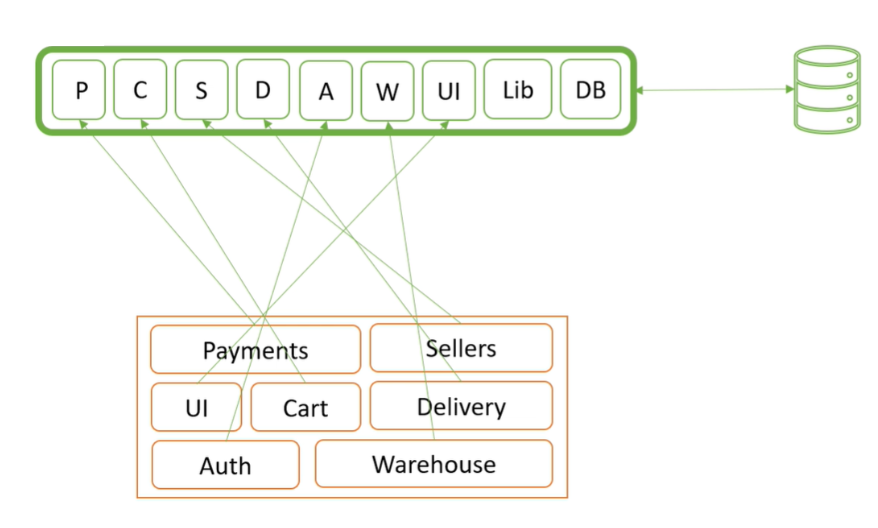
\includegraphics[width=0.7\linewidth]{figures/01_basics/monolithics_apps_oops.png}
\caption{Monolithic app with OOPS}
\label{fig:monolithic_app}
\end{figure}

\subsubsection{Downsides}
As the team grows, some problems starts to coming up with this approach as well:
\begin{itemize}
    \item Another big defect of the monolithic approach is that we are bound to the 
tecnology stack. So if we build a code with Java and Spring, but we need create a 
Machine Learning feature in Python. How can you do this? The solution would be creating a
standalone app to handle this feature. There isn't really a problem with creating a 
standalone feature, but you are defeting the meaning and purpose of a monolithic app. 
    \item Another problem is that it's really easy to break things with this type of 
architecture, because you are never gonna be enterily update of what each person did in the 
code. Thus, if you change some logic, you might break someone's else feature. Sure there're 
some test codes and the second SOLID principle, which is open-closed. But sometimes, even these
are not enough. 
    \item Another major issue is \textbf{scalability}. Let's suppose it's Black Friday: the 
sellings are done constantly and you might be afraid that the system crashes. At this moment 
is necessary to scale the payments and the cart module. The problem with that, is that the 
notification and the Warehouse doesn't need to be modify, but once you changes the Payments and 
the Cart modules, you gonna need to deploy the code again and at this moment the Notification and 
the Warehouse will be idle. A big enterprise such as Amazon would loose a lot of money.  
    \item The bigger the code is, more it takes to be deployed. 
    \item If there's a leak in some part of the system, it's very likely that another part be also
    leaked. Even a small leak in the Warehouse might compromise another module. 
\end{itemize}


\begin{tcolorbox}
    A person started to discuss with me that, the more a code grows, more it becomes difficult to 
    undestand. Mainly when it is done with OOP. Actually, this is not a problem of using OOP or not,
    it's a problem of monolithic approaches. 
\end{tcolorbox}


The solution of all this problems is to use a Microservice architecture. 

\subsection{Microservice architecture}

The main idea is to break down the application into logical components, so that this components
becomes a service on their own. The microservice is the only source of truth of a feature group. 
Now each service will communicate with each other via a set of API calls like REST APIs or 
Remove Procedure calls. 

\subsubsection{Benefits of Microservice}

\begin{itemize}
    \item Now we are not bounded to a single technology stack;
    \item One team can do your work well without worrying about break someone's else feature;
    \item One microservice can be scalled without affecting another entire module;
    \item Iterating deploying and testing is a lot easier. 
    \item The engineers will be working on smaller code bases.  
\end{itemize}


\subsection{Monolithic vs Microservice}

Microservices have a lot of advantages, but it doesn't mean that we should always use Microservices
in one application. 

\subsubsection{Latency}
\begin{itemize}
    \item Of course functions are faster than API calls, thus the 
    Monolithic architecture in more effecient when we talk about communication between modules/
    services. But this delay is not noticed by the user, but in critical services, this might be 
    one aspect to be considered.  
    \item With network calls comes the possibility of network fail. So it increases the 
    complexity of the error handling and retries. 
\end{itemize}

\subsubsection{Backward Compatibility}
\begin{itemize}
    \item If a service makes a change for a mandatory parameter, another service that depends on 
    this one, might break. As an personal opinion, this is not a big issue, because if a service
    creates a new version on every release, than the depending service will not crash. Besides, 
    the same thing might happen in a Monolithic approach: someone might change the parameters of 
    a function, the difference is that the IDE might recognize the error in compilation time. 
    \item To solve this problem some tests are necessary. 
\end{itemize}

\subsubsection{Logging}
\begin{itemize}
    \item If you need to trace logs for a user in monoliths, it is easy to do so as 
    they are all in the same place. But in microservices, for each request from the 
    user there will be multiple service calls.
    \item A way would be storing in each service its individual log. But tracing exactly what 
    happened becomes more difficult. 
    \item A better approach would be to store all the logs in just one central place where they
    can be queried. This is a cost, since you need to build a \textbf{Log Aggregation System} or 
    buy a third-part system license. 
\end{itemize}

\subsubsection{Service Discovery}
    \begin{itemize}
        \item If you are calling multiple services, we need a way to identify where they are hosted.
        \item We could of course hard code this, but that makes it little difficult to change, especially 
        if you have a lot of microservices. 
    \end{itemize}

\subsubsection{Other smaller costs}

\begin{itemize}
    \item We also need a configuration manager system to push configurations into all 
    the nodes of a particular service.
    \item Even though auto scaling is a benefit of microservices, doing it in a controlled 
    manner needs to be done by a system as well.
    \item In monoliths, since all the code and data are in one place, access control is straightforward. ~
    With multiple microservices, access control, security policies, etc., will need to be done for each service repeatedly.
    \item There needs to be a managing infrastructure for all the services that need to asynchronously talk to each other,
    something like a centralized Kafka deployment, which becomes an additional cost.
\end{itemize}

So, there're a lot of components just running to support the microservice architecture. 
For small applications, \textbf{the cost of maintanning this architecture is higher than creating 
the application itself}. However, thinking in a real world scenario, there would be hundrer of 
services working together. The cost of creating the support is negligible compared to the development
of the architecture.  

\subsection{Conclusion}
If you are working on small business or small team and have limited set of features, 
monolithic might be a better approach. However, if you are working on a huge product with
hundreds of microservices, the maintenance cost of microservices will be worthwhile. 


\subsection{Questions}

\begin{itemize}
    \item What is a monolithic architecture?
    \item What are the disadvantages of a monolithic architecture?
    \item What is a microservice architecture? 
    \item What are the advantages of a microservice architecture? 
    \item Compare the monolithic and microservice architecture. 
    \item When is it better to use a monolithic architecture? And microservice? 
    \item Why is it interesting to use OOP? 
\end{itemize}